\subsection{Peters' Scheme for $G^1$ B{\'e}zier surface reconstruction}
\label{subsec:peters}
Although the process of generating a NURBS surface may trivially only seem to consist of placing out the control points near the desired surface location, getting it to assume a specified shape can be quite a task. As generating a topology more complex than a torus \todointern{possible reference to figure above} also requires several NURBS surfaces joined together, one needs to filfill certain requirements in order for it to remain connected. For simple surface continuity ($C^0$), it is enough that the control points and knots on the edges of the two patches are the same as the surface then on both edges follows a 1D--NURBS-curve from these points and knots. As higher-order continuity desired for smooth surfaces creates much more complex requirements, several schemes have been created to automate such tasks.

The approach sometimes referred to as \emph{surface splines} or \emph{G-splines} \cite{eck1996automatic} solves the task of generating a smooth surface by starting from a \emph{control mesh} $\petersControlMesh$ of points, and compute B{\'e}zier surfaces by setting their control points to be linear combinations of the points in $\petersControlMesh$, with the coefficients determined such that the resulting surfaces will be \emph{tangent plane continous}, or $G^1$, or other desired degrees of smoothness. 

One such scheme is the scheme of Peters, described in \cite{peters1992constructing}, which starts from an unstructured mesh of polygonal faces, and creates from the location and connectivity of its vertices a $G^1$--continous surface. This means that the normal vector to the plane is countinous, resulting in a smooth surface without sharp corners. The process consists of two steps, described below for a mesh of quadrilateral faces (quads), for which it also was implemented and used for fitting in \citep{eck1996automatic}. However, the scheme could also be applied for a mesh of any mixture of polygons.\tododone[inline]{mention that it's called surface splines or G-splines to create surface from a mesh}

\subsubsection{Mesh refinement}
In the first step, the mesh is refined through two applications of \emph{Doo-Sabin refinement}, as first described in \cite{DooSabin1978subdiv}. In one step of this refinement, a new point $\vec{m}_{ref}$  is created for each vertex $\petersControlMeshVec$ in the control mesh $\petersControlMesh$, for every face $f_{\vec{m}}$ that $\petersControlMeshVec$ corners,  between $\petersControlMeshVec$ and the centroid $\centroidof{f_{\petersControlMeshVec}}$ (the average position of its vertices) of the bordering face $f_{\petersControlMeshVec}$. The refined mesh $\petersControlMesh^{ref}$ then consists of all these created points. Mathematically, for the faces $\petersFaces$, with face ${\hat{f}}$ having vertices $V_{\hat{f}}$:

\begin{align}
\petersControlMesh^{(ref)} =& \lbrace \petersControlMeshVec_{ref} \suchthat\petersControlMeshVec_{ref} = \alpha\petersControlMeshVec + (1-\alpha)\centroidof{f} \suchthat f \in \facesof{\petersControlMeshVec} \suchthat
\\ \notag &
 \suchthat \petersControlMeshVec \in \petersControlMesh, \alpha \in (0,1) \rbrace
\\
\where \qquad\qquad \centroidof{\hat{f}} =& \text{average}(\petersControlMeshVec_{\hat{f}})_{\petersControlMeshVec_{\hat{f}} \in \verticesof{\hat{f}}}
\\
\text{and} \qquad\qquad F_{\vec{\hat{m}}} =& \left\lbrace \hat{f} \suchthat \vec{\hat{m}} \in \verticesof{\hat{f}}	\right\rbrace
\end{align}
where $\alpha$ is a smoothening parameter, controlling the sharpness of the corners and edges, which we for simplicity set to $1/2$, to get a simple midpoint.

Thus, in every refinement step on an $n$--gon, $n$ vertices are created, giving 4 vertices for a quad in the original control mesh. These are then joined up with the neighbours on the quad to form a smaller quad, and with the neighbouring points from the same vertex on the neighbouring quads, forming a quad along each edge, and an $n$--gon around each original vertex, where $n$ is the number of quads that the original cornered. After two refinements, we thus get a mesh of vertices $\petersPatchPoints$ that consists mainly of quads, with some possible other-$n$--gons around the vertices of the original mesh $\petersControlMesh$. The mesh and the resulting structure after two subdivisions can be seen in \autoref{fig:petersSubDivide}b.\todointern{maybe fancy peter's scheme picture, alt the one in EckHoppe for what the thingymajong looks like after 2x ref.}

\begin{figure}
	\centering
	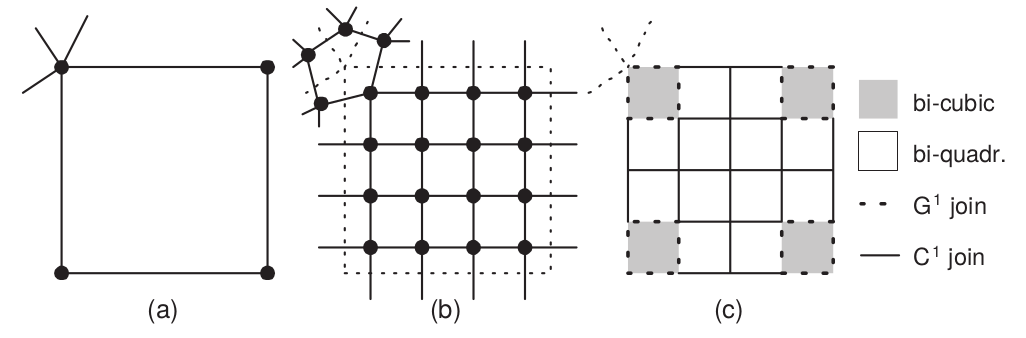
\includegraphics[width = \textwidth]{Pictures/NURBS/petersQuad_to_patches.png}
	\caption{The subdivision step in Peter's scheme. a): A quad in the original mesh, with edges and vertices marked out. Note that there are 5 edges connecting the top-left corner, making this a non-regular mesh corner. b): The mesh resulting from two Doo-Sabin subdivisions. The mesh is regular, except for around the original mesh corners with other than 4 edges. In the case of the top-left corner, the 5 edges result in a pentagon. c): The resulting \Bez patch structure. The surface is at least $G^1$ continous everywhere. Picture taken from \cite{eck1996automatic}.}
	\label{fig:petersSubDivide}
\end{figure}

\subsubsection{Bezier patch creation}
In this step, we create one B{\'e}zier patch for every vertex in the double refined mesh $\petersControlMesh$. 

Since we now have on each original quad a $4 \times 4$ grid of vertices, with each original quad edge having will be $4$ vertices on each side, we can see that most of the cells will locally be in a regular grid, in the sense that it will have $8$ local neighbours ($4$ along the edges of the double refined quads, and $4$ along the diagonals of the doubly refined quads), see \autoref{fig:petersSubDivide} for details. 
For those cells, we can now create biquadratic tensor splines that meet $G^1$ along the edges and corners; that is, the tensor product of one quadratic spline in one of the regular mesh directions and one in the other. As shown and proven in \cite{peters1992constructing}, this is achieved by creating a \Bez patch for each vertex (see \autoref{fig:petersSubDivide}c for the patch structure) with 8 \Bez control points at the average position of the center vertex and each of the 8 neighbours, and one on the center vertex itself.


%as following (see [\todointern[inline]{ref to figure with names on points, EckHoppe or Peters}] for nomenclature):
%%
%\begin{equation}
%
%\end{equation}
%%
\todointern[inline]{For final version: math formulae for \Bez points from regular mesh points}

The exceptions which might not be placeable in a regular mesh is now the points residing on the corners of the original quads. This comes from the fact that at quad corners, we may have any number of quads meeting, starting from 3. \todointern{possible example fig?} As mentioned above, this forms an $n$--gon ($n \geq 3$) in the doubly refined mesh, for whose vertices we cannot apply the same procedure as in the regular mesh example above. 

The solution to how to create \Bez patches over these corners is to place a bicubic (of polynomial order 3) \Bez patch for each corner point, placing the \Bez control points in such a way that they both match up smoothly to the regular mesh patches, and to the other neighbouring patches, and that all match up smoothly about the original mesh corner. For bicubic \Bez patches, there are more than enough degrees of freedom to do this, and in Peters' scheme, this is done by letting each \Bez control point, just as in the regular case, be a linear combination of all the neighbouring points, but here taking into account all the vertices that were generated from the Doo--Sabin refinement with the original corner vertex, that is, all vertices that are neighbouring a corner on the $n$--gon. The formulae are derived and proved to result in a $G^1$ surface in \cite{peters1992constructing}.%, and can be found in 
\todointern[inline]{insert appendix}. 

To summarize, Peters' scheme is a mathematical algorithm for creating biquadratic and bicubic \Bez patches that join with $G^1$ continuity, from a mesh of polygons. The \Bez control points defining the patches are all created from linear combinations of the vertices in the polygonal mesh, with an inbetween step to the refined mesh points (that is, the refined mesh points are linear combinations of the original mesh points, and they then form linear combinations to create the \Bez control points).

\tododone[inline]{Erik: inserted stuff here}
%In this section we will cover the following, referring to \cite{peters1992constructing}:
%\begin{itemize}
%\item How we go from polygonal faces to a set of mesh control points. "patch points", specifying that we're talking about quads, and that we then get 16
%\item That for each of these 16 points, we will make a small B{\'e}zier patch
%\item That if we define the B{\'e}zier control points of these patches in a special way, as described in appendix XYZ \todointern{TODO: create this appendix, or change this to refer to paper for coefficients}, we get a surface that is $G^1$ continous
%\item Maybe describe that we then need for every one of these B{\'e}zier patches the locations of the neighbours
%\item That the location of a point on the surface defined by parameters $\vec{s} = (u,v)$ depends on the B{\'e}zier control points, whose linear dependence on the "patch points" give us coefficients on these "patch points" of the location described by the parameters, as can be seen in \autoref{fig:PetersPoints}
%
%\end{itemize}
\begin{figure}

\missingfigure{Graphical description of all those different points in Peters' Scheme}
\label{fig:PetersPoints}
\caption{The points in Peters' Scheme. As clearly seen in the figure above, this scheme is self-explanatory.}
\end{figure}